\chapter{Methodological approach}
- (3h) Writing Process: Go through markdown notes (prepare writing)
- (2h+) Refactoring: Start Camunda Modeler (see whether it works)
	-> Look at results for next steps


\section{Motivation and Procedure}
% 
% What we did so far: Transition
% 

%
% Goals and Priority
%


% Primary Goal is to do the Refactoring Process

% TODO: Formulate this caveat after writing the business case
	% Business Case will not be covered, technical debt will not be estimated.
	% - But: Software Project will be transformed in future
	% - Thus: By the detection of internal problems coupled future development,
	% 	refactoring seems to be self-evident.

% Note: Reworking the entire Application is not in the scope of the thesis

% Secondary Goals - Discussion part
Whereas primary ...





% ------------------------------------------------------------------------
% Hypotheses
% ------------------------------------------------------------------------
Based on these goals -> constucted following hypotheses.

During the practical work, 
	the thesis will try to validate two types of hypotheses.


% ------------------------------------------------------------------------
% Transition: Short Overview of Procedure
% ------------------------------------------------------------------------

\section{Analysis: Detecting Code Smells}

% Introduction Paragraph
The following part of this chapter moves on to describe in greater detail detection code smells within the software system. It provides a brief overview of the methods used for detection and mentions the prevalence of sonargraph as the main suite of software products utilized in the detection activities. Moreover, this section provides some clarifications necessary to comprehend certain methods to be chosen over others.

% Catalogue
Out of 24 code smells that are examined throughout Martin Fowler's book on refactoring, only 10 are chosen to be included in the detection work. Further, the 2 smells \emph{refused bequest} and \emph{data clumps} were discarded, as their focus on inheritance and data structures respectively, are not utilized in the code. In order to revisit the code smell catalog with their corresponding explanation, refer to (sec:...)
 

% Restrictions
There exists several reasons that have led to the decision of restricting the amount of smells for this section. First, it is not the scope of the thesis to find every code smell in the codebase. Finding and evaluating each smell that is known in literature would be a tedious task, as there are no automatic tools available for the python programming language, as will be discussed in a later part of this section. Hence, it suffices, if some smells that are prevalent have been detected. In addition, it is also advantageous to only focus on the most prominent smells. Very niche smells could distract from improving the quality of the entire code base, as well as provide less of possibilities to make generalizations.

% Metrics based
Many tools have been created to automatically or semi-automatically detect code smells (Menshawy, p.1). In the context of our paper, the code smells are detected semi-automatically using a metric-based approach. This approach measures source code elements and takes decisions based on threshold values (Menshawy, p.4) It is fulfills two requirements necessary for the following work. On the one hand, it to a certain degree contains automation, making it much more efficient in comparison to manual approaches. On the contrary, it can be used for the python programming language, which is essential in the software system at hand. Menshawy points out (p.3) that with metrics approach does not provide metrics for every code smells. Nevertheless, for the eight smells the thesis is focussing on, as will be seen afterwards, an appropriate metric was found.

% Automation based
Using a detection approach based on automated tools would have been more attractive, but unfortunately not possible.  It is the most used approach (Menshawy, p.2), its availability is however highly dependent on the programming language the software system is written in (Menshawy, p.3). By looking at Menshawy's research (p.3) on most cited tools, it can be observed that a significant difference exists between java programming language, which was supported  by 48\% of the tools, whereas the python programming language being only supported by 4\%.
In addition, by researching automated tools appropriate for python, it was evident that at this moment of time, the offering is insufficient for to accomplish a sound detection strategy. 

% Manual approach
In the beginning, the author has also considered following a manual approach. In contrast to automation, the manual detection relies on human perception of smells by applying predefined guidelines (Menshawy, p.3). It is characterized as highly time-consuming and prone to human error. Therefore, when comparing this approach to a metrics-based, it is a less desirable way for detecting smells and was subsequently discarded as a detection technique.

% Visualization
Another detection approach that has not yet been mentioned, is using visualization. Although it only is used to detect a subset of smells, visualization had been used in two occurrences throughout the thesis. First, it had been used to get a broad overview of the code base, which helped the author as an orientation. Second, it was used [... Add coupling + cohesion]

% Intro Sonargraph
The detection of code smells relied heavily on a code analyzer tool called sonargraph. It demonstated to be extremely useful in the detection of code smells, by its ability to compute and list metrics of the software system. Countless metrics offered a diversity of selection, analyzing both on the basis of the entire project and individual modules. By reading through the the provided explanations of the metric an appropriate metric could be found for all of the desired code smells relevant for the thesis.

% Explorer + Metrics
Compared to other software solutions, sonargraph was chosen for several reasons. Altough its entire product suite is not, its graphical application "Explorer" was free to use. For the thesis it provided many ways to make observations about the code base, including numerical and visual methods. All the tools needed to compute metrics were restricted in this free application of the product family. In contrast, the detection of code duplication was not included within "Explorer". Nevertheless, altough unsure about the amount, it was possible to renew a trial period multiple times. Hence, in order to recreate this method one must be aware of this restriction. Another noteworthy benefit of using sonargraph during the detection, was its ability to observe the entire project,  and not just at individual files. This was essential for metrics taking account of dependencies between modules. In addition, it was beneficial not to rely on a multitude of software tools, by having just one software.



\begin{figure}[htp]
    \centering
    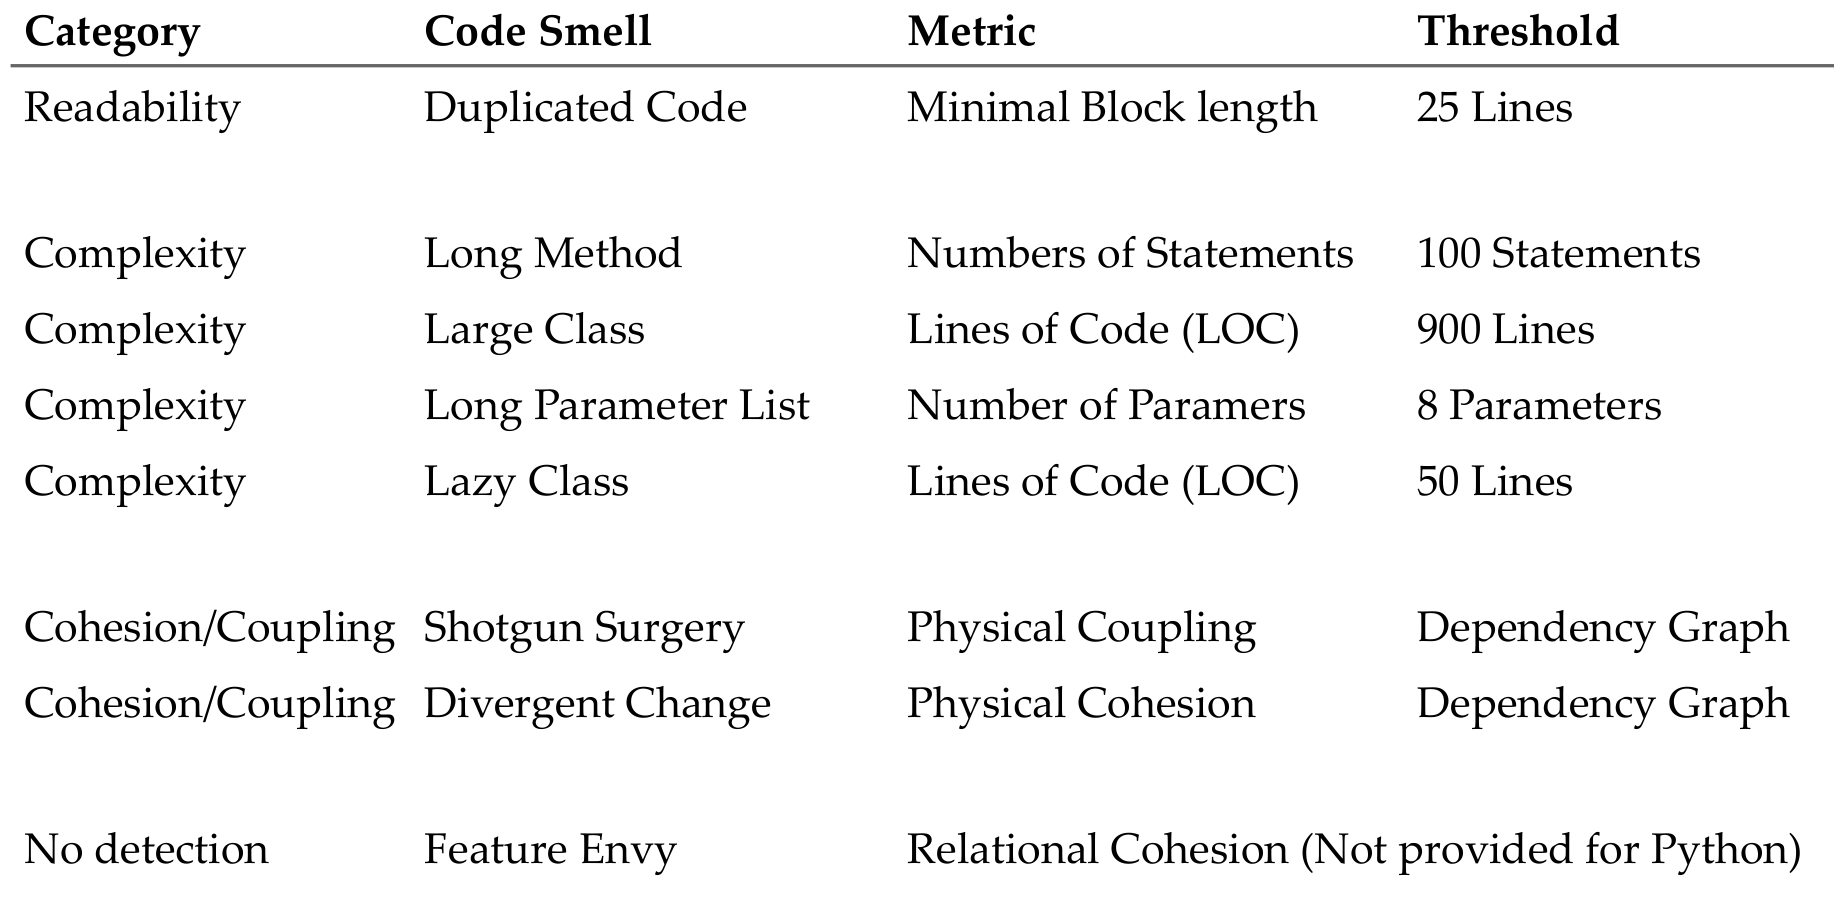
\includegraphics[width=\textwidth]{./assets/smell_overview}
    \caption{Metrics without prioritization}
\end{figure}
% Table
The above table presents for each code smell a corresponding metric. In addition, for some metrics, a threshold value is given. When the threshold value is surpassed, there is an indication that this code smell exists in the software system.

% Subgroups
Individual metrics are categorized into three subgroups, named after the quality attribute they best represent. More importantly, however, this distinction is made, as each of the group differs in regard to how a metric results in a smell detected. 

% Duplicated Code -> Automated
Duplicate code particularly differs from the other smells, due to it being detected automatically. Previously, it was stated that it was difficult to find appropriate tools to detect code smells, due to lack of availability.
In the case of code duplication, this is however readily available because detecting code duplication can be done language agnostic. In order to detect duplication of code in programs, the software does not need to understand the programming language. For instance, this same mechanism could be applied to other types of text that are not code.

% Complexity -> Threshold
Half of the code smells, in the subgroup called complexity, follow a typical metrics based approach. The threshold value indicate when a code smell is potentially present. Notably, all the metrics in this category involve counting of some sorts. In particular, the smells are detected by counting the number of statements, lines of codes, and numbers of parameters of methods. Prioritization of given smells can be done by comparing the extent of how much a given threshold value is surpassed. Similarly, code smells can be discarded if the associated metric does not surpass the threshold value. 


% Cohesion/Coupling -> Dependency graph
[Don't know yet]
- For Shotgun Surgery and Divergent change, a dependency graph will be used in addition to the metric.
- Sonargraph does not provide a threshold value.
	-> This allows to evaluate the amount of dependencies in relation to the entire project in order to see any outlying behavior


\section{Testing: Framework}
% Transition
In the section that follows, it will be argued that testing is a fundamental part of the refactoring process. In the context of the thesis, it moves on to describe in greater detail the challenges that occur when testing a cyber physical system. In the section that follows, the methods used for testing 
will be outlined, which draw together previously discussed challenges.

\myparagraph{Importance of Testing in a Refactoring Process}

% Importance of Tests
Moving on now to consider, in what ways, testing plays an important role in the refactoring process. In order to understand the significance, it is appropriate to return to the subject of Martin Fowler's definition. According to his definition, refactoring does not alter the external behavior of code {fowler2018}. It was pointed out in the theoretical part of this paper that by not changing the features of the program, programmers can alleviate the risks associated with changing the codebase, which mainly includes the creation of new bugs. Because ofthis, one can immediately understand how testing is required during refactoring. In more concrete terms, if we want to find out whether the behavior of the code base did not alter, we use testing to confirm this notion. 

% False perception
Further, confirming an unaltered state of code behavior is vital to verify the improvement of code quality. Disregarding testing is likely to result in a false perception of code quality, as bugs are not taken in consideration. In other words, testing can ensure that the software system is in a better state than before, given the quality metrics have improved.

% Mistakes
Allen Holub demonstrates these risks with the statement that "Refactoring without tests is like crossing a busy street blindfolded" (Allen Holub). Similarly, Fowler [p.~59]{fowler2018} argues, mistakes naturally occur and are not a problem if caught quickly. Further, in regard to refactoring he mentions the significance of self-testing code, which allows making it much safer to add new features without breaking anything.

\myparagraph{Testing Cyber Physical Systems}



% CPS Challenges
Having defined the importance, it is now necessary to explain the present challenges given that our software system being a cyber-physical sytem (CPS). The different characteristics of CPS also needs to be taken into account when determining the methodology of testing these systems. Robots and other cyber-physical systems react to information from the physical worlds and must operate safely even in the presence of uncertainties {geissvolkermaria}. In such a dynamic real-world environment, Kapur {kapurpulkit2020} describes testing, whether a robot will behave as expected, as a time consuming and complicated task for developers. {raikumar2010} points out the the challenge of the heterogenous nature of CPS, making it difficult to verify and validate the software systems. Similarly, {abbaspourasadollah2015} mentions that defining the boundaries and physical limitations of the test landscape is a challenge in testing a CPS. Another limitation in CPS testing is using an automated semi-automated method. Here, the efficacy of testing is limited by the element its hardware components. Testing is then dependent to hardware operating approprietly and therefore including the prominence of physical motions subject to considerable time necessary for each test run. The lack of available software that mitigate these challenges poses a substantial limitation on the testing within our context. Some challenges for instance could be mitigated by using a physics-based simunation that mimics the real-world envirionment. Simulations do exist in practice, but are unavailable for the present software system. 


% Software test -> Manual test
In general, there is a high interest to use automated testing, as manual testing is more likely to produce errors {turlea2019}.  The levels of CPS software testing contains verifying software, hardware, network, and the integration of all these components to work as a single system {abbaspourasadollah2015}. Despite the advantages of automated test, the fact needs to be considered that for the software system at hand, none of these software tests are available. As a result, developing a testing suite for the software system scratch would certainly be out of the scope of this thesis. 

% One advantage
In fact, there exists an advantage of manual testing that is particular to CPS. Indeed, the physical nature of CPS allows the manual testing through visual observation. Moreover, this benefit is especially apparent when taking into account that our software project is focussing on managing entire processes. In other words, we have the ability to detect for any change in behavior by testing a specific process. 

% Justification
Both the lack of software tests and the ability to visually observe behavior changes were the primary motivations that manual testing was chosen as the preferred method. It is still less reliable compared to software testing, but adequate to reach the aims of the thesis. This is due to the fact that, while not guaranteeing the equality of the entire software system, this method can decently predict the equivalence of the software needed for specific processes used for testing. One key factor in this approach is the selection of one or multiple processes that best cover most of the software system. Consequently, the interactions among the individual components can be examine, delivering benefits similar to integration testing. All in all, this approach does not provide the same degree of assurance as comprehensive unit and integration testing. Nevertheless, it is an approach that suits the preconditions within our context. Specifically, we can to a certain degree assume that we did not alter the external behavior within the scope of specific processes. 

\myparagraph{Method selection}

% Transition
As indicated previously, testing for this thesis will be done manually by means of observing an entire process of the CPS. Methods are selected that strive to be able to test objectively and in a routinized manner. Camunda Modeler is used to automate the business processes and the Gherkin Language is used to formulate requirements. Using Camunda Modeler provides objectivity by having a standardized way to run processes. Similarly, the Gherkin language offers a way to objectively formulate requirements. In combination, these tools deliver a procedure to reduce ambiguity, which is essential in order to capture any cues in observable changes. Having this standardized approach allows us to alleviate some of the shortcoming of manual testing, while also reducing human error.

% What we have
=== Visualization: Camunda Screenshot ===
Even though there are no software tests available, multiple business processes in using the a BPMN representation have already been implemented for the present software system. These representation in the form of files are what is being executed by camunda to allow the automation of the processes. 

[We use this process]
- Because it covers all components and major parts of the software system, 

Accordingly, this software solution sequentially does HTTP requests that would otherwise have been done manually. Performing these requests manually would not only be very tedious, but also introduce ambiguity. In addition, the BPMN notation used by Camunda Modeler allows us to visually inspect at which part of the process one currently is when running it. This is a fundamental feature, when trying to find out where a current issue might be located.


% Gherkin Explanation
Gherkin on the other hand is not a software solution. Instead it is a language that is oftentimes used in conjunction with other software tools. Hereby, one can formulate behavior in the form of specifications written in plain text and understandable by humans. It usess a set of special keywords that enables formulating these specifications in a structured way (https://cucumber.io/docs/gherkin/reference/). We can then validate whether the software does what the specifications say. The validation is oftentimes done with writing related software tools. However, in our context this will be done manually. Consequently, using the gherkin language we are able to objectively check whether the current codebase still fulfills the specification in a form that is human readable and can also be routinely repeated in a standardized way. 

=== Visualization: Gherkin as code syntax ===

Language
- Feature: 
	High-level description of Application
- Scenario Steps: 
	Action to be performed by a user
	Expected Results of the action
- Scenario Syntax
	Given (preconditions)
	When (user action)
	Then outcome)
	And (multiple statements)

As seen in the specifications above, one can observe multiple prerequisites that are necessary due to having hardware. This amount of detail is critical when wanting to reproduce this process at a later time. Even though, some specifications might seem self-evident, only then we can diminish the ambiguity associated with testing CPS. 

% Optional: DEBUGGING
% - Previous stated tool is what we use to periodically check AFTER we did refactoring
% - There are preventative measure one can take DURING the refactoring. For instance bugs can be caught by trying to run python code, and see whether errors are raised
% - At current time, a lot of issues can be caught during programming itself with modern IDEs
% - With an IDE (Integrated Development Environment) Formatters and static type checkers are also able to catch bugs in the code writing process. 
% - During programming I use the pyright server as a static type checker
% - In order to early detect errors before program execution
% - Advantage is that we do not need to tediously run code all the time, but can catch them before running.
% - Don't need to run code to see malfunctions within the code
% - No errors obviously do not mean that there are no bugs. There could still be unexpected behavior.
% 	-> This is especially the case with python (statically typed language, polymorphism) == Means debugging alone would not suffice, testing is key



\section{Measurment: Success}

\section{Implementation: Refactor}

\section{Extra Activities}

\section{Limitations and justification}
